% $Header: /u/gcmpack/manual/s_phys_pkgs/text/exch2.tex,v 1.10 2004/03/15 20:11:56 afe Exp $
% $Name:  $

%%  * Introduction
%%    o what it does, citations (refs go into mitgcm_manual.bib, 
%%      preferably in alphabetic order)
%%    o Equations 
%%  * Key subroutines and parameters
%%  * Reference material (auto generated from Protex and structured comments)
%%    o automatically inserted at \section{Reference} 


\section{exch2: Extended Cubed Sphere \mbox{Topology}}
\label{sec:exch2}


\subsection{Introduction}

The \texttt{exch2} package is an extension to the original cubed
sphere topological configuration that allows more flexible domain
decomposition and parallelization.  Cube faces (also called
subdomains) may be divided into any number of tiles that divide evenly
into the grid point dimensions of the subdomain.  Furthermore, the
individual tiles may be run on separate processors in different
combinations, and whether exchanges between particular tiles occur
between different processors is determined at runtime.  This
flexibility provides for manual compile-time load balancing across a
relatively arbitrary number of processors. \\

The exchange parameters are declared in
\filelink{pkg/exch2/W2\_EXCH2\_TOPOLOGY.h}{pkg-exch2-W2_EXCH2_TOPOLOGY.h}
and assigned in
\filelink{pkg/exch2/w2\_e2setup.F}{pkg-exch2-w2_e2setup.F}. The
validity of the cube topology depends on the \texttt{SIZE.h} file as
detailed below.  Both files are generated by Matlab scripts in
\texttt{utils/exch2/matlab-topology-generator}; see Section
\ref{sec:topogen} for details on creating alternate topologies.  The
default files provided in the release configure a cubed sphere
topology of six tiles, one per subdomain, each with 32$\times$32 grid
points, all running on a single processor.  Pregenerated examples of
these files with alternate topologies are provided under
\texttt{utils/exch2/code-mods} along with the appropriate
\texttt{SIZE.h} file for single-processor execution.

\subsection{Invoking exch2}

To use exch2 with the cubed sphere, the following conditions must be
met: \\

$\bullet$ The exch2 package is included when \texttt{genmake2} is run.  The
  easiest way to do this is to add the line \texttt{exch2} to the
  \texttt{profile.conf} file -- see Section \ref{sect:buildingCode}
  for general details. \\

$\bullet$ An example of \texttt{W2\_EXCH2\_TOPOLOGY.h} and
  \texttt{w2\_e2setup.F} must reside in a directory containing code
  linked when \texttt{genmake2} runs.  The safest place to put these
  is the directory indicated in the \texttt{-mods=DIR} command line
  modifier (typically \texttt{../code}), or the build directory.  The
  default versions of these files reside in \texttt{pkg/exch2} and are
  linked automatically if no other versions exist elsewhere in the
  link path, but they should be left untouched to avoid breaking
  configurations other than the one you intend to modify.\\

$\bullet$ Files containing grid parameters, named
  \texttt{tile}???\texttt{.mitgrid} where ??? is \texttt{001} through
  \texttt{006} (one per subdomain), must be in the working directory
  when the MITgcm executable is run.  These files are provided in the
  example experiments for cubed sphere configurations with
  32$\times$32 cube sides and are non-trivial to generate -- please
  contact MITgcm support if you want to generate files for other
  configurations. \\

$\bullet$ As always when compiling MITgcm, the file \texttt{SIZE.h}
  must be placed where \texttt{genmake2} will find it.  In particular
  for the exch2, the domain decompositin specified in \texttt{SIZE.h}
  must correspond with the particular configuration's topology
  specified in \texttt{W2\_EXCH2\_TOPOLOGY.h} and
  \texttt{w2\_e2setup.F}.  Domain decomposition issues particular to
  exch2 are addressed in Section \ref{sec:topogen}: ``Generating
  Topology Files for exch2''; a more general background on the subject
  relvant to MITgcm is presented in Section
  \ref{sect:specifying_a_decomposition}: ``Specifying a
  decomposition''.\\

As of the time of writing the following examples use exch2 and may be
used for guidance:

\begin{verbatim}
verification/adjust_nlfs.cs-32x32x1
verification/adjustment.cs-32x32x1 
verification/aim.5l_cs
verification/global_ocean.cs32x15
verification/hs94.cs-32x32x5
\end{verbatim}




\subsection{Generating Topology Files for exch2}
\label{sec:topogen}

Alternate cubed sphere topologies may be created using the Matlab
scripts in \texttt{utils/exch2/matlab-topology-generator}. Running the
m-file \texttt{driver} from the Matlab prompt (without passing any
function parameters) generates exch2 topology files
\texttt{W2\_EXCH2\_TOPOLOGY.h} and \texttt{w2\_e2setup.F} in the
working directory and displays via Matlab a figure of the topology.
The other m-files in the directory are subroutines of \texttt{driver}
and should not be run except for development purposes. \\

The parameters that determine the dimensions and topology of the
generated configuration are nr, nb, ng, tnx and tny, and all are
assigned early in the script.

The first three determine the size of the subdomains (cube faces) and
hence the size of the overall domain.  Each one determines the number
of grid points, and therefore the resolution, along the subdomain
sides in a ``great circle'' around each axis of the cube.  At the time
of this writing MITgcm requires these three parameters to be equal,
but they provide for future releases of MITgcm to accomodate different
resolutions around the axes to allow (for example) greater resolution
around the equator.\\

The parameters tnx and tny determine the dimensions of the tiles into
which the subdomains are decomposed, and must evenly divide the
integer assigned to nr, nb and ng.  The result is a rectangular tiling
of the subdomain.  Figure \ref{fig:24tile} shows one possible topology
for a twenty-four tile cube, and figure \ref{fig:12tile} shows one for
twelve tiles. \\

\begin{figure}
\begin{center}
 \resizebox{4in}{!}{
  \includegraphics{part6/s24t_16x16.ps}
 }
\end{center} 
\caption{Plot of cubed sphere topology with a 32$\times$32 grid and
twenty-four tiles (tnx=16, tny=16)
} \label{fig:24tile}
\end{figure}

\begin{figure}
\begin{center}
 \resizebox{4in}{!}{
  \includegraphics{part6/s12t_16x32.ps}
 }
\end{center} 
\caption{Plot of cubed sphere topology with a 32$\times$32 grid and
twelve tiles (tnx=16, tny=32)
} \label{fig:12tile}
\end{figure}

Tiles can be selected from the topology to be omitted from being
allocated memory and processors.  This kind of tuning is useful in
ocean modeling for omitting tiles that fall entirely on land.  The
tiles omitted are specified in the file \texttt{blanklist.txt} by
their tile number in the topology, separated by a newline. \\






\subsection{Key Variables}

The descriptions of the variables are divided up into scalars,
one-dimensional arrays indexed to the tile number, and two and three
dimensional arrays indexed to tile number and neighboring tile.  This
division actually reflects the functionality of these variables: the
scalars are common to every part of the topology, the tile-indexed
arrays to individual tiles, and the arrays indexed to tile and
neighbor to relationships between tiles and their neighbors.

\subsubsection{Scalars}

The number of tiles in a particular topology is set with the parameter
\texttt{NTILES}, and the maximum number of neighbors of any tiles by
\texttt{MAX\_NEIGHBOURS}.  These parameters are used for defining the
size of the various one and two dimensional arrays that store tile
parameters indexed to the tile number.\\

The scalar parameters \varlink{exch2\_domain\_nxt}{exch2_domain_nxt}
and \varlink{exch2\_domain\_nyt}{exch2_domain_nyt} express the number
of tiles in the x and y global indices.  For example, the default
setup of six tiles has \texttt{exch2\_domain\_nxt=6} and
\texttt{exch2\_domain\_nyt=1}.  A topology of twenty-four square (in
gridpoints) tiles, four (2x2) per subdomain, will have
\texttt{exch2\_domain\_nxt=12} and \texttt{exch2\_domain\_nyt=2}.
Note that these parameters express the tile layout to allow global
data files that are tile-layout-neutral and have no bearing on the
internal storage of the arrays.  The tiles are internally stored in a
range from \texttt{1,bi} (in the x axis) and y-axis variable
\texttt{bj} is generally ignored within the package.

\subsubsection{Arrays Indexed to Tile Number}

The following arrays are of size \texttt{NTILES}, are indexed to the
tile number, and the indices are omitted in their descriptions.

The arrays \varlink{exch2\_tnx}{exch2_tnx} and
\varlink{exch2\_tny}{exch2_tny} express the x and y dimensions of each
tile.  At present for each tile \texttt{exch2\_tnx=sNx} and
\texttt{exch2\_tny=sNy}, as assigned in \texttt{SIZE.h}.  Future
releases of MITgcm are to allow varying tile sizes.

The location of the tiles' Cartesian origin within a subdomain are
determined by the arrays \varlink{exch2\_tbasex}{exch2_tbasex} and
\varlink{exch2\_tbasey}{exch2_tbasey}.  These variables are used to
relate the location of the edges of the tiles to each other.  As an
example, in the default six-tile topology (the degenerate case) each
index in these arrays are set to 0.  The twenty-four, 32x32 cube face
case discussed above will have values of 0 or 16, depending on the
quadrant the tile falls within the subdomain.  The array 
\varlink{exch2\_myFace}{exch2_myFace} contains the number of the
cubeface/subdomain of each tile, numbered 1-6 in the case of the
standard cube topology.

The arrays \varlink{exch2\_txglobalo}{exch2_txglobalo} and
\varlink{exch2\_txglobalo}{exch2_txglobalo} are similar to
\varlink{exch2\_tbasex}{exch2_tbasex} and
\varlink{exch2\_tbasey}{exch2_tbasey}, but locate the tiles within the
global address space, similar to that used by global files.

The arrays \varlink{exch2\_isWedge}{exch2_isWedge},
\varlink{exch2\_isEedge}{exch2_isEedge},
\varlink{exch2\_isSedge}{exch2_isSedge}, and
\varlink{exch2\_isNedge}{exch2_isNedge} are set to 1 if the indexed
tile lies on the edge of a subdomain, 0 if not.  The values are used
within the topology generator to determine the orientation of
neighboring tiles and to indicate whether a tile lies on the corner of
a subdomain.  The latter case indicates special exchange and numerical
handling for the singularities at the eight corners of the cube.
\varlink{exch2\_nNeighbours}{exch2_nNeighbours} contains a count of
how many neighboring tiles each tile has, and is used for setting
bounds for looping over neighboring tiles.
\varlink{exch2\_tProc}{exch2_tProc} holds the process rank of each
tile, and is used in interprocess communication.

\subsubsection{Arrays Indexed to Tile Number and Neighbor}

The following arrays are all of size \texttt{MAX\_NEIGHBOURS} $\times$
\texttt{NTILES} and describe the orientations between the the tiles.

The array \texttt{exch2\_neighbourId(a,T)} holds the tile number for
each of the $n$ neighboring tiles.  The neighbor tiles are indexed
\texttt{(1,MAX\_NEIGHBOURS} in the order right to left on the north
then south edges, and then top to bottom on the east and west edges.
Maybe throw in a fig here, eh?

The \texttt{exch2\_opposingSend\_record(a,T)} array holds the index c
in \texttt{exch2\_neighbourId(b,$T_{n}$)} that holds the tile number T.
In other words, 
\begin{verbatim}
   exch2_neighbourId( exch2_opposingSend_record(a,T),
                      exch2_neighbourId(a,T) ) = T
\end{verbatim}
and this provides a back-reference from the neighbor tiles.

The arrays \varlink{exch2\_pi}{exch2_pi},
\varlink{exch2\_pj}{exch2_pj}, \varlink{exch2\_oi}{exch2_oi},
\varlink{exch2\_oj}{exch2_oj}, \varlink{exch2\_oi\_f}{exch2_oi_f}, and
\varlink{exch2\_oj\_f}{exch2_oj_f} specify the transformations in
exchanges between the neighboring tiles.  The dimensions of
\texttt{exch2\_pi(t,N,T)} and \texttt{exch2\_pj(t,N,T)} are the
neighbor ID \textit{N} and the tile number \textit{T} as explained
above, plus the transformation vector {\em t }, of length two.  The
first element of the transformation vector indicates the factor by
which variables representing the same vector component of a tile will
be multiplied, and the second element indicates the transform to the
variable in the other direction.  As an example,
\texttt{exch2\_pi(1,N,T)} holds the transform of the i-component of a
vector variable in tile \texttt{T} to the i-component of tile
\texttt{T}'s neighbor \texttt{N}, and \texttt{exch2\_pi(2,N,T)} hold
the component of neighbor \texttt{N}'s j-component.

Under the current cube topology, one of the two elements of
\texttt{exch2\_pi} or \texttt{exch2\_pj} for a given tile \texttt{T}
and neighbor \texttt{N} will be 0, reflecting the fact that the vector
components are orthogonal.  The other element will be 1 or -1,
depending on whether the components are indexed in the same or
opposite directions.  For example, the transform dimension of the
arrays for all tile neighbors on the same subdomain will be [1,0],
since all tiles on the same subdomain are oriented identically.
Vectors that correspond to the orthogonal dimension with the same
index direction will have [0,1], whereas those in the opposite index
direction will have [0,-1].


{\footnotesize
\begin{verbatim}
C      exch2_pi          :: X index row of target to source permutation 
C                        :: matrix for each neighbour entry.            
C      exch2_pj          :: Y index row of target to source permutation 
C                        :: matrix for each neighbour entry.            
C      exch2_oi          :: X index element of target to source 
C                        :: offset vector for cell-centered quantities  
C                        :: of each neighbor entry.                     
C      exch2_oj          :: Y index element of target to source 
C                        :: offset vector for cell-centered quantities  
C                        :: of each neighbor entry.                     
C      exch2_oi_f        :: X index element of target to source 
C                        :: offset vector for face quantities           
C                        :: of each neighbor entry.                     
C      exch2_oj_f        :: Y index element of target to source 
C                        :: offset vector for face quantities           
C                        :: of each neighbor entry.                     
\end{verbatim}
}



\subsection{Key Routines}



\subsection{References}
